\section{Token}
Ein Token, ist eine Errungenschaft welcher ein Benutzer beim Erfolgreichen Abschluss einer Quest bekommen kann. Dadurch soll vorallem die Motivation der Benutzer gesteigert werden. 

\subsection{Variablen in der token.java}

\begin{lstlisting}[language=JAVA]
	private String title;		//Titel des Tokens
	private String initPath;	//Pfad zum Packages Ordner 
	private String relPath;		//relativer Pfad zum Token
	private String description;	//Beschreibung des Tokens
	private String imagePath;	//Pfad zum Bild

\end{lstlisting}
Diese Variablen sind alle mithilfe von Gettern und Settern erreichbar.

\subsection{Odnersturktur der Tokens}
Tokens befinden sich in einem Ordner mit dem Namen "`tokens"' in einem Package. Ein hier definiertes Token kann in einer Quest des aktuellen Packages zugewiesen werden. Tokens können somit nicht Package-Übergreifend aufgerufen werden.

\begin{figure}[h] 
  \centering
     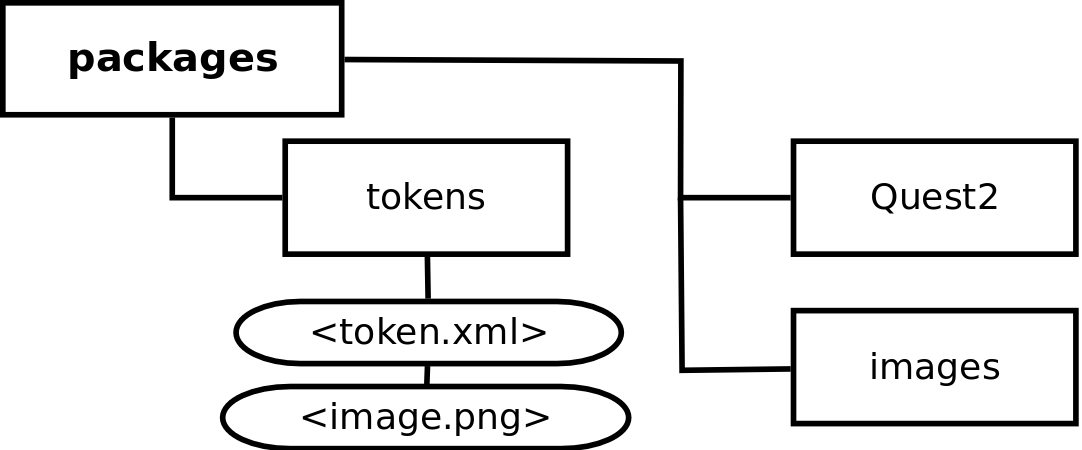
\includegraphics[width=0.5\textwidth]{./media/images/quest/token.png}
  \caption{Struktur einer Ordner}
  \label{fig:struct_token}
\end{figure}

Das Bild welches für ein Token verwendet wird, kann auch in spezifischen Ordnerstruktur verschachtelt sein. Jedoch muss dies bei der Erstellung des "<token.xml"> berücksichtigt werden.